\documentclass[8pt]{beamer}

\usetheme{psy9511}

\usepackage{graphicx}
\usepackage{pgfplots}
\usepackage{pgfplotstable}
\usepackage{varwidth}
\usepackage{xcolor}

\usetikzlibrary{arrows}
\usetikzlibrary{arrows.meta}
\usetikzlibrary{calc}
\usetikzlibrary{matrix}

\date{23.09.24}
\title{Introduksjon til maskinlæring}
\subtitle{Bildegjenkjenning med Python og Tensorflow}
\author{Esten H. Leonardsen}

\colorlet{model1}{red}
\colorlet{model2}{green}
\colorlet{model3}{orange}

\def\nodesize{14pt}
\colorlet{nodefill}{green!20}

\begin{document}
	\newcommand{\cnnchannel}[4]{
		\def\cellsize{0.15}
		\foreach \i in {1,...,#3} {
			\foreach \j in {1,...,#3} {
				\pgfmathsetmacro{\ioffset}{(\i - floor(#3 / 2))}
				\pgfmathsetmacro{\joffset}{(\j - floor(#3 / 2))}
				\node[
					draw=black,
					fill=green!20,
					minimum width=\cellsize cm,
					minimum height=\cellsize cm,
					anchor=south east,
					inner sep=0pt
				] (#4\i\j) at ({#1 - (\ioffset * \cellsize)}, {#2 - (\joffset * \cellsize)}) {};

			}
		}
	}

	\newcommand{\cnnlayer}[5]{
		\pgfmathsetmacro{\rounded}{floor(#4 / 2)}
		\message{\rounded}
		\foreach \c in {1,...,#4} {
			\pgfmathsetmacro{\offset}{\c - 1 - \rounded}
			\cnnchannel{#1 + \offset * 0.1}{#2 - \offset * 0.1}{#3}{#5\c}
		}
	}

	 \begin{frame}
	 	\maketitle
	 \end{frame}

	\begin{frame}{Plan for dagen}
		\vfill
		Teori:
		\begin{itemize}
			\item Hva er en statistisk læringsmodell?
			\item Hva er en kost-funksjon?
			\item Hvordan trener vi en statstisk læringsmodell?
			\item Hvordan fungerer et (dypt) kunstig nevralt nettverk?
			\item Hvordan fungerer et konvolusjonelt nevralt nettverk (for klassifikasjon)?
			\item Hva er transfer learning?
			\item Hva er overtilpasning, og hvordan unngår vi det?
		\end{itemize}
		Praktisk workshop:
		\begin{enumerate}
			\item Sette opp et Python-miljø i Google Colab
			\item Predikere med et ferdigtrent konvolusjonelt nevralt nettverk
			\item Retrene en klassifikator for blomsterarter
			\item Hvis tid, forbedre klassifikatoren
		\end{enumerate}
		\vfill
	\end{frame}

	\begin{frame}{Motivasjon}
		\centering
		\begin{tikzpicture}
			\node[] at (-5.25, -3) {};
			\node[] at (5.25, 3) {};

			\visible<1>{
				\node[] at (-4.3, 0) {
					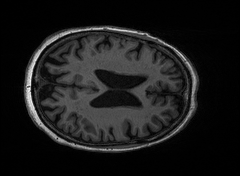
\includegraphics[width=1.8cm]{data/control_1.png}
				};
				\node[] at (-4.15, -2) {
					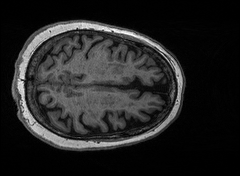
\includegraphics[width=1.8cm]{data/control_2.png}
				};
				\node[] at (-2.1, -0.75) {
					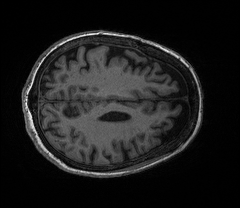
\includegraphics[width=1.8cm]{data/control_3.png}
				};
				\node[] at (-4.05, 2) {
					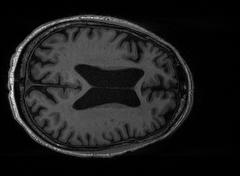
\includegraphics[width=1.8cm]{data/control_4.png}
				};
				\node[] at (-1.7, 1.25) {
					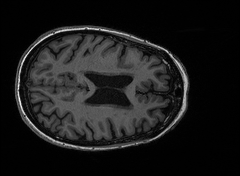
\includegraphics[width=1.8cm]{data/control_0.png}
				};

				\node[] at (1, -1.75) {
					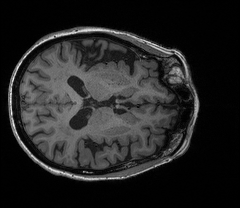
\includegraphics[width=1.8cm]{data/patient_0.png}
				};

				\node[] at (3.5, -1.95) {
					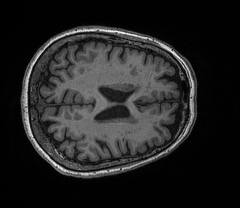
\includegraphics[width=1.8cm]{data/patient_1.png}
				};
				\node[] at (1.25, 0.25) {
					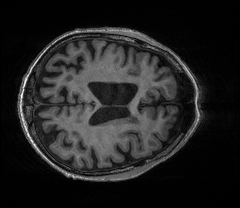
\includegraphics[width=1.8cm]{data/patient_3.png}
				};
				\node[] at (3.75, 0) {
					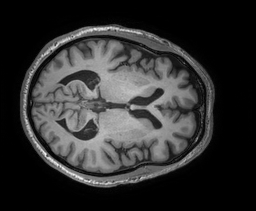
\includegraphics[width=1.8cm]{data/patient_2.png}
				};

				\node[] at (2.5, 2.1) {
					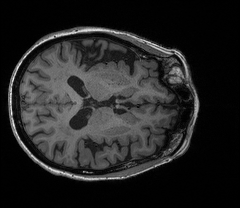
\includegraphics[width=1.8cm]{data/patient_0.png}
				};

				\draw[very thick, red] (0.15,3.4) -- (-0.85, -3.7);
				\node[] at (-1.7, -3.5) {Kontroller};
				\node[] at (0, -3.5) {Pasienter};
			}
			\visible<2>{
				\node[font=\footnotesize\selectfont] at (0, 0) {
					\url{https://drive.google.com/file/d/1CLgpFaXDukFpBmhHHzPCZdtuXtecXqPO/view}
				};
			}
			\visible<3>{
				\node[inner sep=0pt, draw=black] at (0, 0) {
					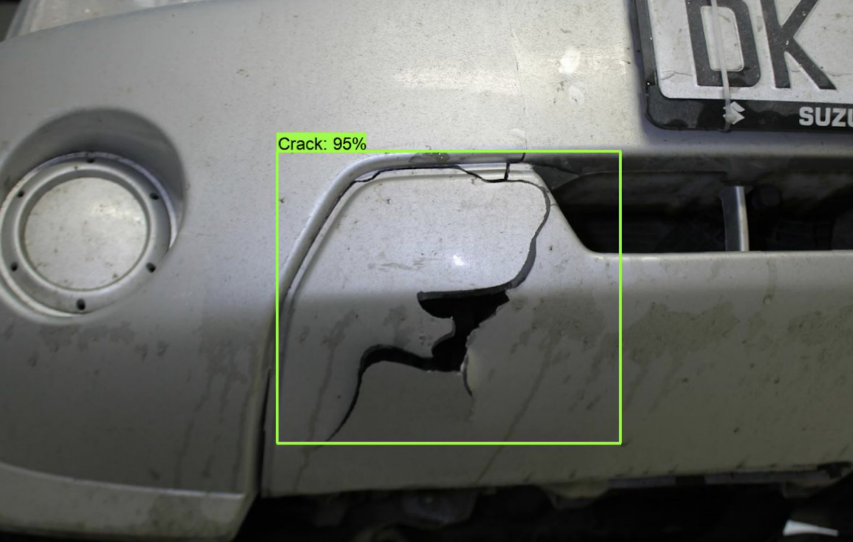
\includegraphics[width=7cm]{data/gjensidige.png}
				};
			}
			\visible<4>{
				\node[inner sep=0pt, draw=black] at (0, 0) {
					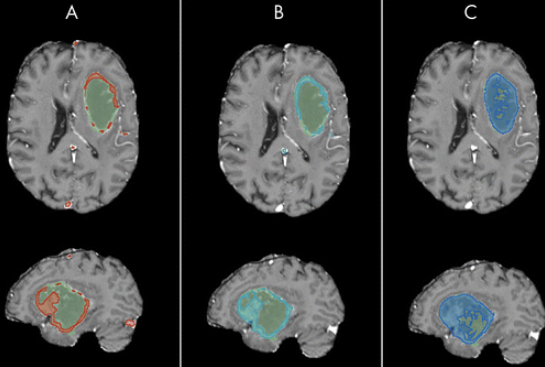
\includegraphics[width=7cm]{data/glioblastoma.png}
				};
			}
			\visible<5>{
				\node[inner sep=0pt, draw=black] at (0, 0) {
					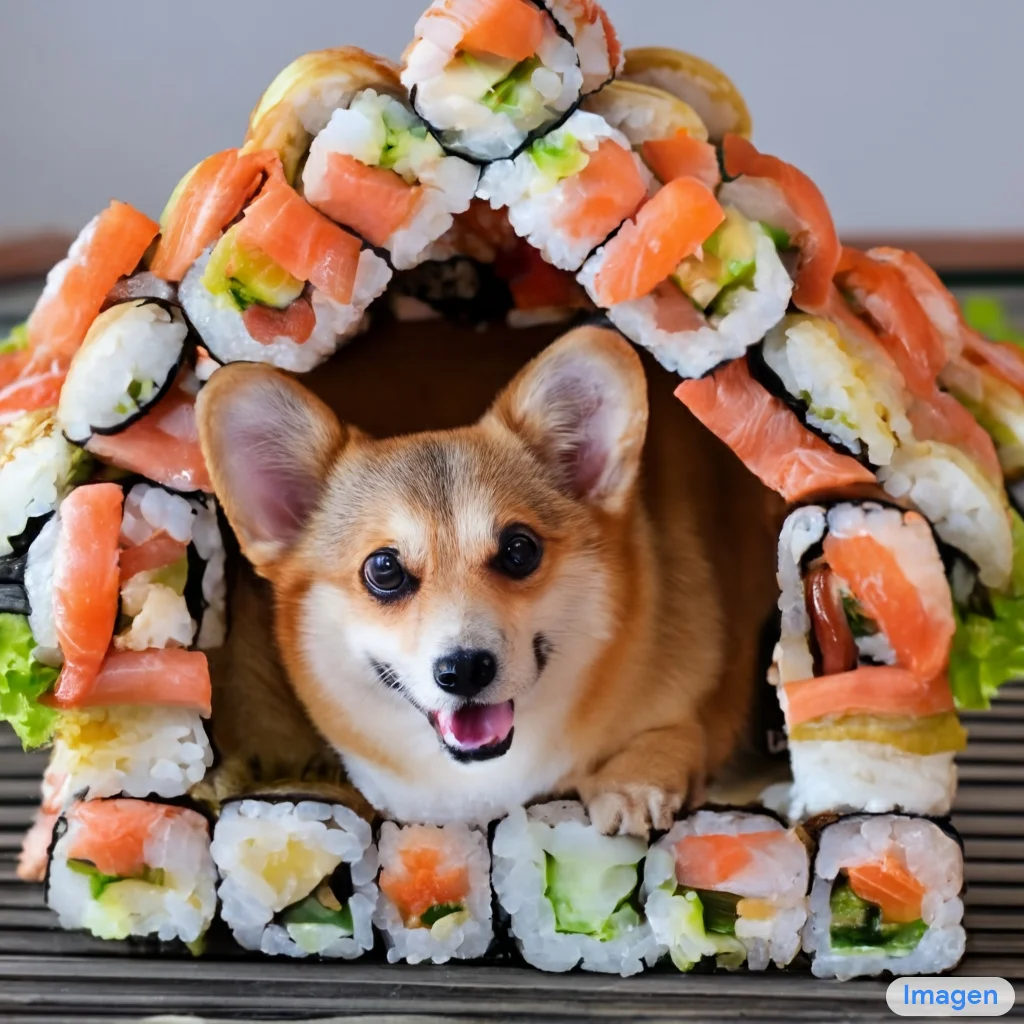
\includegraphics[width=7cm]{data/dog-in-sushihouse.png}
				};
			}
		\end{tikzpicture}
	\end{frame}

	\section{Statistisk læring}

	\newcommand{\losstrace}[2]{
		\addplot[dashed] coordinates {
			(#1, 3500000 + #1 * 30000)
			(#1, #2)
		};
	}

	\newcommand{\olsplot}[1]{
		\begin{tikzpicture}
			\begin{axis}[
				xlabel=$m^2$,
				ylabel=NOK,
				ytick={4000000, 5000000, 6000000, 7000000, 8000000},
				yticklabels={4M, 5M, 6M, 7M, 8M},
				scaled y ticks=false,
				xtick pos=bottom,
				ytick pos=left,
				xmin=30,
				xmax=90,,
				ymin=3500000,
				ymax=8800000,
				height=6.5cm,
				width=10cm
			]
				\addplot[
					only marks,
					mark size=3pt,
					mark options={draw=black, fill=cyan}
				] coordinates {
					(72, 5127379)
					(50, 4552170)
					(45, 4486654)
					(62, 5709276)
					(53, 4634912)
					(81, 8388570)
					(44, 4828170)
					(78, 7557770)
					(37, 4016520)
					(73, 6572351)
				};

				\ifnum#1=1
					\addplot[red, thick] coordinates {
						(57, 3500000)
						(57, 8800000)
					};
				\fi

				\ifnum#1>1
					\ifnum#1<10
						\addplot[green] coordinates {
							(0, 3500000)
							(100, 6500000)
						};
					\fi
				\fi

				\ifnum#1=3
					\addplot[red] coordinates {
						(0, 6000000)
						(100, 6000000)
					};
					\addplot[orange] coordinates {
						(0, 706495)
						(100, 8909658)
					};
				\fi

				\ifnum#1>3
					\ifnum#1<7
						\draw[dashed] (axis cs: 78, 3500000) -- (axis cs: 78, 8800000);
					\fi
				\fi

				\ifnum#1>4
					\ifnum#1<10
						\addplot[
							only marks,
							mark size=3pt,
							mark options={draw=green, fill=white},
							fill opacity=0
						] coordinates {
							(78, 3500000 + 78 * 30000)
						};
					\fi
				\fi

				\ifnum#1<9
					\ifnum#1>4
						\node[anchor=west] at (axis cs: 79, 5840000) {\footnotesize{$\hat{y}$}};
					\fi

					\ifnum#1>5
						\node[anchor=west] at (axis cs: 79, 7557770) {\footnotesize{$y$}};
					\fi
				\fi

				\ifnum#1>6
					\ifnum#1<10
						\losstrace{78}{7557770}
					\fi
				\fi

				\ifnum#1=8
					\node[anchor=west] at (axis cs: 78, 6698885) {\footnotesize{$\ell=(y-\hat{y})^2$}};
				\fi

				\ifnum#1=9
					\losstrace{72}{5127379}
					\losstrace{50}{4552170}
					\losstrace{45}{4486654}
					\losstrace{62}{5709276}
					\losstrace{53}{4634912}
					\losstrace{81}{8388570}
					\losstrace{44}{4828170}
					\losstrace{37}{4016520}
					\losstrace{73}{6572351}
				\fi

				\ifnum#1=10
					\addplot[green] coordinates {
						(0, 3000000)
						(100, 7500000)
					};
				\fi

				\coordinate (center) at (axis cs: 60, 3500000);
			\end{axis}
		\end{tikzpicture}
	}

	\newsavebox{\olsdata}
	\sbox{\olsdata}{\olsplot{0}}
	\newsavebox{\olsprediction}
	\sbox{\olsprediction}{\olsplot{1}}
	\newsavebox{\olssingle}
	\sbox{\olssingle}{\olsplot{2}}
	\newsavebox{\olsmulti}
	\sbox{\olsmulti}{\olsplot{3}}
	\newsavebox{\olsnewx}
	\sbox{\olsnewx}{\olsplot{4}}
	\newsavebox{\olsyhat}
	\sbox{\olsyhat}{\olsplot{5}}
	\newsavebox{\olsy}
	\sbox{\olsy}{\olsplot{6}}
	\newsavebox{\olsloss}
	\sbox{\olsloss}{\olsplot{7}}
	\newsavebox{\olsse}
	\sbox{\olsse}{\olsplot{8}}
	\newsavebox{\olsmse}
	\sbox{\olsmse}{\olsplot{9}}
	\newsavebox{\olsupdate}
	\sbox{\olsupdate}{\olsplot{10}}

	\begin{frame}{Statistisk læring: Modeller}
		\centering
		\begin{tikzpicture}
			\node[] at (-5.25, -3.75) {};
			\node[] at (5.25, 3.75) {};

			\visible<1>{
				\node[draw=black, inner sep=0pt] at (0, 0) {
					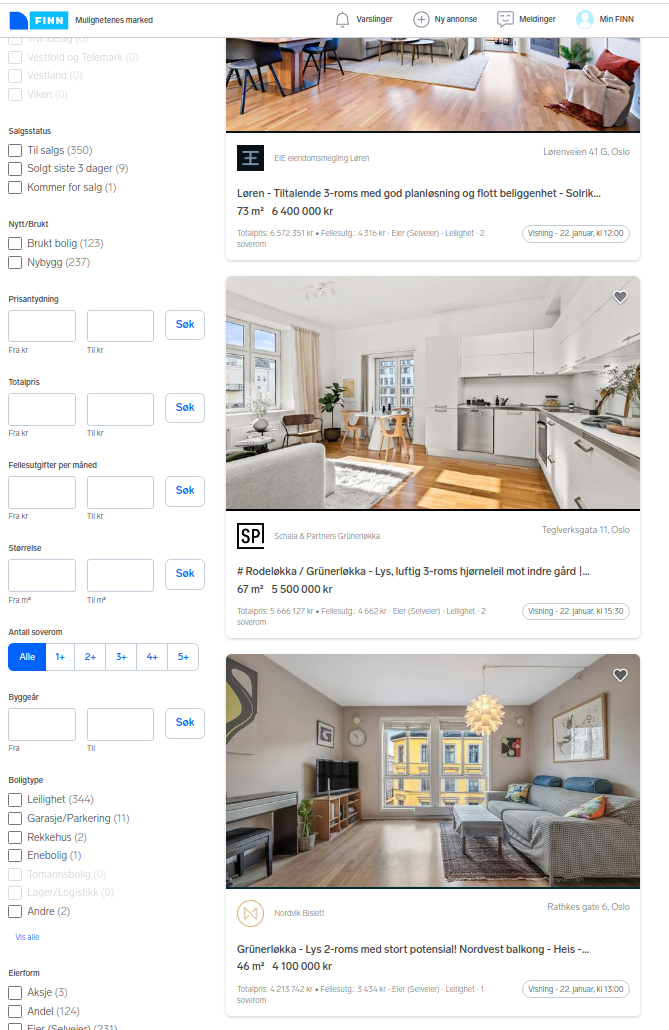
\includegraphics[height=7cm]{data/finn.png}
				};
			}
			\visible<2>{
				\node[] at (0, 0) {
					\begin{tabular}{|c|c|}
						\hline
						\textbf{$m^2$}&\textbf{Price}\\
						\hline
						72&5.127.379\\
						\hline
						50&4.552.170\\
						\hline
						45&4.486.654\\
						\hline
						62&5.709.276\\
						\hline
						53&4.634.912\\
						\hline
						81&8.388.570\\
						\hline
						44&4.828.170\\
						\hline
						78&7.557.770\\
						\hline
						37&4.016.520\\
						\hline
						73&6.572.351\\
						\hline
					\end{tabular}
				};
			}
			\visible<3-4>{
				\node[] at (-0.4, 0.6) {
					\usebox{\olsdata}
				};
			}
			\visible<4>{
				\node[] at (0, -2.75) {
					$\hat{y}=f(x)$
				};
			}
			\visible<5>{
				\node[] at (-0.4, 0.6) {
					\usebox{\olsprediction}
				};
				\node[] at (0, -2.75) {
					$\hat{y}=f($\textcolor{red}{$x$}$)$
				};
			}
			\visible<6>{
				\node[align=left, text width=9cm] at (0, 0) {
					\textbf{Hva er en statistisk læringsmodell?}
					\begin{itemize}
						\item En matematisk konstruksjon (ofte en formel) som representerer forholdet mellom input $x$ og output $y$
						\item En funksjonell enhet som, gitt ny data $x$ er i stand til å predikere nye utfall $y$
					\end{itemize}
				};
			}
		\end{tikzpicture}
	\end{frame}

	\begin{frame}{Statistisk læring: Kost-funksjoner}
		\centering
		\begin{tikzpicture}
			\node[] at (-5.25, -3.75) {};
			\node[] at (5.25, 3.75) {};

			\visible<1>{
				\node[] at (0, -2.75) {
					$\hat{y}=$ $b$ $+$ $w$$x$
				};
			}
			\visible<1-2>{
				\node[] at (-0.4, 0.6) {
					\usebox{\olsdata}
				};
			}
			\visible<2>{
				\node[] at (0, -2.75) {
					$\hat{y}=$ \textcolor{red}{$b$} $+$ \textcolor{red}{$w$}$x$
				};
			}
			\visible<3,5>{
				\node[] at (-0.4, 0.6) {
					\usebox{\olssingle}
				};
			}
			\visible<3-5,11-13>{
				\node[] (m2) at (0, -2.75) {
					\textcolor{green}{$\hat{y}=3500000 + 30000x$}
				};
			}
			\visible<4,13>{
				\node[] at (-0.4, 0.6) {
					\usebox{\olsmulti}
				};
				\node[anchor=east, text=red] (m1) at ($ (m2.west) + (-0.25, 0) $) {
					$\hat{y}=6000000 + 0x$
				};

				\node[anchor=west, text=orange] (m3) at ($ (m2.east) + (0.25, 0) $) {
					$\hat{y}=706495 + 82031x$
				};
			}
			\visible<6>{
				\node[] at (-0.4, 0.6) {
					\usebox{\olsnewx}
				};
			}
			\visible<6-10>{
				\node[text=green] at (0, -2.75) {
					$\hat{y}=3500000 + 30000 * 78$
				};
			}
			\visible<7>{
				\node[] at (-0.4, 0.6) {
					\usebox{\olsyhat}
				};
			}
			\visible<8>{
				\node[] at (-0.4, 0.6) {
					\usebox{\olsy}
				};
			}
			\visible<9>{
				\node[] at (-0.4, 0.6) {
					\usebox{\olsloss}
				};
			}
			\visible<10>{
				\node[] at (-0.4, 0.6) {
					\usebox{\olsse}
				};
			}
			\visible<11-12>{
				\node[] at (-0.4, 0.6) {
					\usebox{\olsmse}
				};
			}
			\visible<11>{
				\node[text=green, anchor=north] at ($ (m2.south) + (0, 0.1) $) {
					$\ell=\dfrac{1}{N}\sum (y - \hat{y})^2$
				};
			}
			\visible<12-13>{
				\node[text=green, anchor=north] at ($ (m2.south) + (0, 0.1) $) {
					$\ell=1.10 \times 10^{13}$
				};
			}
			\visible<13>{
				\node[anchor=north, text=red] at ($ (m1.south) + (0, 0.1) $) {
					$\ell=2.08 \times 10^{13}$
				};

				\node[anchor=north, text=orange] at ($ (m3.south) + (0, 0.1) $) {
					$\ell=4.09 \times 10^{12}$
				};
			}
			\visible<14>{
				\node[align=left, text width=9cm] at (0, 0) {
					\textbf{Hva er en kost-funksjon?}
					\begin{itemize}
						\item En matematisk funksjon som beregner kostnaden av å bruke en gitt modell for å forklare et gitt datasett
						\item En formalisering av oppgaven vi ønsker at modellen skal løse
					\end{itemize}
				};
			}
		\end{tikzpicture}
	\end{frame}

	\begin{frame}{Statistisk læring: Trening}
		\centering
		\begin{tikzpicture}
			\node[] at (-5.25, -3.75) {};
			\node[] at (5.25, 3.75) {};

			\visible<1-5>{
				\node[] at (-0.4, 0.6) {
					\usebox{\olssingle}
				};
			}
			\visible<1-2>{
				\node[] (model) at (0, -2.75) {
					$\hat{y}=$ $b$ $+$ $w$$x$
				};
				\node[] (loss) at (0, -3.25) {
					$\ell=\dfrac{1}{N}\sum (y - \hat{y})^2$
				};
			}
			\visible<2>{
				\node[draw=red, minimum height=0.35cm, thick, minimum width=0.22cm] at ($ (model) - (0.645, 0) $) {};
				\node[draw=red, minimum height=0.35cm, thick, minimum width=0.22cm] at ($ (loss) + (0.61, 0) $) {};
			}
			\visible<3>{
				\node[] (loss) at (0, -3) {
					$\ell=\dfrac{1}{N}\sum (y - (b + wx))^2$
				};
			}
			\visible<4-5>{
				\node[] (loss) at (0, -3) {
					$1.10 \times 10^{13}=\dfrac{1}{N}\sum (y - (3500000 + 30000x))^2$
				};
			}
			\visible<5>{
				\draw[-stealth] ($ (loss.south) - (2.23, -0.2) $) -- ($ (loss.south) - (2.23, 0) $);
				\draw[-stealth] ($ (loss.south) + (0.75, 0.2) $) -- ($ (loss.south) + (0.75, 0) $);
				\draw[-stealth] ($ (loss.north) + (2.03, -0.2) $) -- ($ (loss.north) + (2.03, 0) $);
			}
			\visible<6>{
				\node[] at (-0.4, 0.6) {
					\usebox{\olsupdate}
				};
				\node[] (loss) at (0, -3) {
					$7.24 \times 10^{12}=\dfrac{1}{N}\sum (y - (3000000 + 45000x))^2$
				};
			}
			\visible<7>{
				\node[align=left, text width=9cm] at (0, 0) {
					\textbf{Hvordan trener vi en statistisk læringsmodell?}
					\begin{enumerate}
						\item Estimer prediksjoner for alle datapunkter
						\item Beregn kostnaden av disse prediksjonene (ved å sammenligne med fasit)
						\item Kalkuler hvordan parametrene i modellen påvirker kostnaden
						\item Oppdater parametrene i den retningen som minsker kostnaden
					\end{enumerate}
				};
			}
		\end{tikzpicture}
	\end{frame}

	\section{Kunstige nevrale nettverk}

	\newsavebox{\threedimensional}
	\sbox{\threedimensional}{
		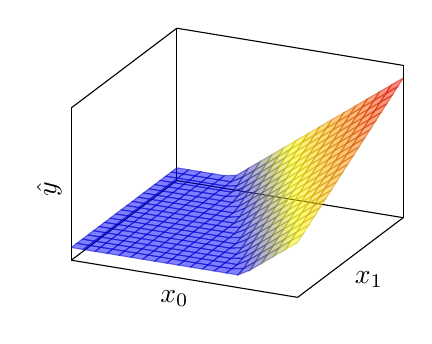
\begin{tikzpicture}[
			declare function = {
				q(\x) = \x - 1;
				Z(\x,\y) = max(0, \x*0.5 + \y*0.25);
			}
		]
			\begin{axis}
			[
				height=5cm,
				ticks=none,
				xlabel=$x_0$,
				ylabel=$x_1$,
				zlabel=$\hat{y}$,
				domain=-1:1,
				samples=20,
			]
				\addplot3 [surf, opacity=0.5] {Z(x,y)};
			\end{axis}
		\end{tikzpicture}
	}

	\begin{frame}{Kunstige nevrale nettverk: Oppbygning}
		\centering
		\begin{tikzpicture}
			\node[] at (-5, 3) {};
			\node[] at (5, -4.5) {};

			\visible<1-2>{
				\node[] at (0, 0) {$\hat{y}=wx+b$};
			}
			\visible<1-3>{
				\node[
					circle,
					draw=black,
					fill=nodefill,
					minimum size=\nodesize,
					inner sep=0pt
				] (n) at (0, 1.5) {};
				\node[] (x) at (-1.5, 1.5) {$x$};
				\node[] (b) at (0, 2.5) {$b$};
				\node[] (y) at (1.5, 1.5) {$\hat{y}$};

				\draw[->] (x) -- (n) node [midway, above] {$w$};
				\draw[->] (b) -- (n);
				\draw[->] (n) -- (y);
			}
			\visible<2>{
				\draw[] (-2, -1.5) -- (2, -1.5) -- (2, -4) -- (-2, -4) -- (-2, -1.5);

				\draw[very thick, blue!60] (-2, -3.5) -- (2, -1.75);

				\node[anchor=north] at (0, -4.1) {x};
				\node[anchor=south, rotate=90] at (-2.1, -2.75) {$\hat{y}$};
			}
			\visible<3>{
				\node[] at (0, 0) {$\hat{y}=max(0, wx+b)$};

				\draw[->] (x) -- (n) node [midway, above] {$w$};
				\draw[->] (b) -- (n);
				\draw[->] (n) -- (y);

				\draw[] (-2, -1.5) -- (2, -1.5) -- (2, -4) -- (-2, -4) -- (-2, -1.5);
				\draw[very thick, blue!60] (-2, -3.5) -- (0, -3.5) -- (2, -1.75);

				\node[anchor=north] at (0, -4.1) {x};
				\node[anchor=south, rotate=90] at (-2.1, -2.75) {$\hat{y}$};
			}
			\visible<4>{
				\node[
					circle,
					draw=black,
					fill=green!20,
					minimum size=\nodesize,
					inner sep=0pt
				] (n0) at (0, 2) {};
				\node[
					circle,
					draw=black,
					fill=nodefill,
					minimum size=\nodesize,
					inner sep=0pt
				] (n1) at (0, 1) {};
				\node[] (x) at (-1.5, 1.5) {$x$};
				\node[] (y) at (1.5, 1.5) {$\hat{y}$};
				\node[] at (0, 0) {$\hat{y}=max(0, w_0x+b_0)+max(0, w_1x+b_1)$};

				\draw[->] (x) -- (n0) node [midway, above] {$w_0$};
				\draw[->] (x) -- (n1) node [midway, below] {$w_1$};
				\draw[->] (n0) -- (y);
				\draw[->] (n1) -- (y);

				\draw[] (-2, -1.5) -- (2, -1.5) -- (2, -4) -- (-2, -4) -- (-2, -1.5);
				\draw[very thick, blue!60] (-2, -3.5) -- (-0.66, -3.5) -- (0.66, -2.25) -- (2, -3);

				\node[anchor=north] at (0, -4.1) {x};
				\node[anchor=south, rotate=90] at (-2.1, -2.75) {$\hat{y}$};
			}
			\visible<5>{
				\node[align=center, text width=10cm] at (0, -0.75) {
					\textbf{Universal approximation theorem:}\\
					\begin{quotation}
						\centering
						"Any relationship that can be described with a polynomial function can be approximated by a neural network with a single hidden layer."
					\end{quotation}
				};
			}
			\visible<6>{
				\node[
					circle,
					draw=black,
					fill=nodefill,
					minimum size=\nodesize,
					inner sep=0pt
				] (n) at (0, 1.5) {};
				\node[] (x0) at (-1.5, 2) {$x_0$};
				\node[] (x1) at (-1.5, 1) {$x_1$};
				\node[] (b) at (0, 2.5) {$b$};
				\node[] (y) at (1.5, 1.5) {$\hat{y}$};
				\node[] at (0, 0) {$\hat{y}=max(0, w_0x_0+w_1x_1+b)$};

				\draw[->] (x0) -- (n) node [midway, above] {$w_0$};
				\draw[->] (x1) -- (n) node [midway, below] {$w_1$};
				\draw[->] (b) -- (n);
				\draw[->] (n) -- (y);

				\node[] at (0, -2.75) {
					\usebox{\threedimensional}
				};
			}
			\visible<7-11>{
			}
			\visible<7-10>{
				\node[
					circle,
					draw=black,
					fill=nodefill,
					minimum size=\nodesize,
					inner sep=0pt
				] (n00) at (0, 2) {};
				\node[
					circle,
					draw=black,
					fill=nodefill,
					minimum size=\nodesize,
					inner sep=0pt
				] (n01) at (0, 1) {};
			}
			\visible<7>{
				\node[
					circle,
					minimum size=\nodesize,
					inner sep=0pt,
					text depth=0
				] (x) at (-3, 1.5) {\footnotesize{$x$}};

				\draw[->] (x) -- (n00) node [midway, above] {$w_0$};
				\draw[->] (x) -- (n01) node [midway, below] {$w_1$};

				\draw[->] (n00) -- (y);
				\draw[->] (n01) -- (y);

				\def\spacing{-0.1cm}
				\node[anchor=north] at (0, 0) {\tiny{
					\begin{math}
						\begin{alignedat}{5}
							\hat{y} = max(0, w_0x+b_0)+max(0, w_1x+b_1)\\
						\end{alignedat}
					\end{math}
				}};
			}
			\visible<8-9>{
				\node[
					circle,
					draw=black,
					fill=nodefill,
					minimum size=\nodesize,
					inner sep=0pt,
					text depth=0
				] (x) at (-3, 1.5) {\footnotesize{$x$}};

				\draw[->] (x) -- (n00) node [midway, above] {$w^0_0$};
				\draw[->] (x) -- (n01) node [midway, below] {$w^0_1$};

				\def\spacing{-0.1cm}
				\node[anchor=north] at (0, 0) {\tiny{
					\begin{math}
						\begin{alignedat}{5}
							\hat{y} = max(0, w^1_{0,0}*max(0, w^0_{0,0}*x+b_{0,0})+w^1_{1,0}*max(0, w^0_{0,1}*x+b_{1,0})+b_1)\\
						\end{alignedat}
					\end{math}
				}};
			}
			\visible<8-12>{
				\node[
					circle,
					draw=black,
					fill=nodefill,
					minimum size=\nodesize,
					inner sep=0pt,
					text depth=0
				] (y) at (3, 1.5) {\footnotesize{$\hat{y}$}};
			}
			\visible<8-10>{
				\draw[->] (n00) -- (y) node [midway, above] {$w^1_0$};
				\draw[->] (n01) -- (y) node [midway, below] {$w^1_0$};
			}
			\visible<9>{
				\node[text depth=0] at (-3, 0.3) {\textcolor{red}{Input}};
				\node[text depth=0] at (0, 0.3) {\textcolor{red}{Hidden}};
				\node[text depth=0] at (3, 0.3) {\textcolor{red}{Output}};
			}
			\visible<10-12>{
				\node[
					circle,
					draw=black,
					fill=green!20,
					minimum size=\nodesize,
					inner sep=0pt,
					text depth=0
				] (x0) at (-3, 2) {\footnotesize{$x_0$}};
				\node[
					circle,
					draw=black,
					fill=green!20,
					minimum size=\nodesize,
					inner sep=0pt,
					text depth=0
				] (x1) at (-3, 1) {\footnotesize{$x_1$}};
			}
			\visible<10>{
				\draw[->] (x0) -- (n00);
				\draw[->] (x0) -- (n01);
				\draw[->] (x1) -- (n00);
				\draw[->] (x1) -- (n01);

				\node[anchor=north] at (0, 0) {\tiny{
					\begin{math}
						\begin{alignedat}{5}
							\hat{y} &= max(0, &&w^1_{0,0}*max(0, w^0_{0,0}*x_0+w^0_{1,0}*x_{1}+b_{0,0})+\\[\spacing]
							& &&w^1_{1,0}*max(0, w^0_{0,1}*x_0+w^0_{1,1}*x_{1}+b_{0,1})+\\[\spacing]
							& &&b_1)&&\\
						\end{alignedat}
					\end{math}
				}};
			}
			\visible<11>{
				\node[
					circle,
					draw=black,
					fill=green!20,
					minimum size=\nodesize,
					inner sep=0pt
				] (n00) at (0, 2.5) {};
				\node[
					circle,
					draw=black,
					fill=green!20,
					minimum size=\nodesize,
					inner sep=0pt
				] (n01) at (0, 1.5) {};
				\node[
					circle,
					draw=black,
					fill=green!20,
					minimum size=\nodesize,
					inner sep=0pt
				] (n02) at (0, 0.5) {};

				\draw[->] (x0) -- (n00);
				\draw[->] (x0) -- (n01);
				\draw[->] (x0) -- (n02);
				\draw[->] (x1) -- (n00);
				\draw[->] (x1) -- (n01);
				\draw[->] (x1) -- (n02);

				\draw[->] (n00) -- (y);
				\draw[->] (n01) -- (y);
				\draw[->] (n02) -- (y);

				\node[anchor=north] at (0, 0) {\tiny{
					\begin{math}
						\begin{alignedat}{5}
							\hat{y} &= max(0, &&w^1_{0,0}*max(0, w^0_{0,0}*x_0+w^0_{1,0}*x_{1}+b_{0,0})+\\[\spacing]
							& &&w^1_{1,0}*max(0, w^0_{0,1}*x_0+w^0_{1,1}*x_{1}+b_{0,1})+\\[\spacing]
							& &&w^1_{2,0}*max(0, w^0_{0,2}*x_0+w^0_{1,2}*x_{1}+b_{0,2})+\\[\spacing]
							& &&b_1)&&\\
						\end{alignedat}
					\end{math}
				}};
			}
			\visible<12>{
				\node[
					circle,
					draw=black,
					fill=green!20,
					minimum size=\nodesize,
					inner sep=0pt
				] (n00) at (-1, 2.5) {};
				\node[
					circle,
					draw=black,
					fill=green!20,
					minimum size=\nodesize,
					inner sep=0pt
				] (n01) at (-1, 1.5) {};
				\node[
					circle,
					draw=black,
					fill=green!20,
					minimum size=\nodesize,
					inner sep=0pt
				] (n02) at (-1, 0.5) {};

				\node[
					circle,
					draw=black,
					fill=green!20,
					minimum size=\nodesize,
					inner sep=0pt
				] (n10) at (1, 2.5) {};

				\node[
					circle,
					draw=black,
					fill=green!20,
					minimum size=\nodesize,
					inner sep=0pt
				] (n11) at (1, 1.5) {};
				\node[
					circle,
					draw=black,
					fill=green!20,
					minimum size=\nodesize,
					inner sep=0pt
				] (n12) at (1, 0.5) {};

				\draw[->] (x0) -- (n00);
				\draw[->] (x0) -- (n01);
				\draw[->] (x0) -- (n02);
				\draw[->] (x1) -- (n00);
				\draw[->] (x1) -- (n01);
				\draw[->] (x1) -- (n02);

				\draw[->] (n00) -- (n10);
				\draw[->] (n00) -- (n11);
				\draw[->] (n00) -- (n12);
				\draw[->] (n01) -- (n10);
				\draw[->] (n01) -- (n11);
				\draw[->] (n01) -- (n12);
				\draw[->] (n02) -- (n10);
				\draw[->] (n02) -- (n11);
				\draw[->] (n02) -- (n12);

				\draw[->] (n10) -- (y);
				\draw[->] (n11) -- (y);
				\draw[->] (n12) -- (y);

				\node[anchor=north] at (0, 0) {\tiny{
					\begin{math}
						\begin{alignedat}{5}
							\hat{y} &= max(0, &&w^2_{0,0}*max(0, &&w^1_{0,0}*max(0, w^0_{0,0}*x_0+w^0_{1,0}*x_{1}+b_{0,0})+\\[\spacing]
							& && &&w^1_{1,0}*max(0, w^0_{0,1}*x_0+w^0_{1,1}*x_{1}+b_{0,1})+\\[\spacing]
							& && &&w^1_{2,0}*max(0, w^0_{0,2}*x_0+w^0_{1,2}*x_{1}+b_{0,2})+\\[\spacing]
							& && &&b_{1,0})+\\[\spacing]
							& &&w^2_{1,0}*max(0, &&w^1_{0,1}*max(0, w^0_{0,0}*x_0+w^0_{1,0}*x_{1}+b_{0,0})+\\[\spacing]
							& && &&w^1_{1,1}*max(0, w^0_{0,1}*x_0+w^0_{1,1}*x_{1}+b_{0,1})+\\[\spacing]
							& && &&w^1_{2,1}*max(0, w^0_{0,2}*x_0+w^0_{1,2}*x_{1}+b_{0,2})+\\[\spacing]
							& && &&b_{1,1})+\\[\spacing]
							& &&w^2_{2,0}*max(0, &&w^1_{0,2}*max(0, w^0_{0,0}*x_0+w^0_{1,0}*x_{1}+b_{0,0})+\\[\spacing]
							& && &&w^1_{1,2}*max(0, w^0_{0,1}*x_0+w^0_{1,1}*x_{1}+b_{0,1})+\\[\spacing]
							& && &&w^1_{2,2}*max(0, w^0_{0,2}*x_0+w^0_{1,2}*x_{1}+b_{0,2})+\\[\spacing]
							& && &&b_{1,2})+\\[\spacing]
							& &&b_2)&&\\
						\end{alignedat}
					\end{math}
				}};
			}
			\visible<13>{
				\node[align=left, text width=9cm] at (0, 0) {
					\textbf{Hvordan fungerer et (dypt) kunstig nevralt nettverk?}\\
					\begin{itemize}
						\item Kunstige nevroner som hver for seg beregner en enkel, ikke-lineær funksjon kombineres i en komputasjonell graf
						\item Grafen som helhet kan beregne arbitrært komplekse sammenhenger mellom input og output
					\end{itemize}

				};
			}

		\end{tikzpicture}
	\end{frame}

	\section{Konvolusjonelle nevrale nettverk}

	\begin{frame}{Konvolusjonelle nevrale nettverk: Bildeinput}
		\centering
		\begin{tikzpicture}[ampersand replacement=\&]
			\node[] at (-5.25, -3.5) {};
			\node[] at (5.25, 3.5) {};

			\visible<1-3>{
				\node[
					circle,
					draw=black,
					fill=green!20,
					minimum size=\nodesize,
					inner sep=0pt,
					text depth=0
				] (x0) at (-3, 0.5) {\footnotesize{$x_0$}};
				\node[
					circle,
					draw=black,
					fill=green!20,
					minimum size=\nodesize,
					inner sep=0pt,
					text depth=0
				] (x1) at (-3, -0.5) {\footnotesize{$x_1$}};
			}
			\visible<1-2,6>{
				\node[
					circle,
					draw=black,
					fill=green!20,
					minimum size=\nodesize,
					inner sep=0pt
				] (n00) at (-1, 1) {};
				\node[
					circle,
					draw=black,
					fill=green!20,
					minimum size=\nodesize,
					inner sep=0pt
				] (n01) at (-1, 0) {};
				\node[
					circle,
					draw=black,
					fill=green!20,
					minimum size=\nodesize,
					inner sep=0pt
				] (n02) at (-1, -1) {};

				\node[
					circle,
					draw=black,
					fill=green!20,
					minimum size=\nodesize,
					inner sep=0pt
				] (n10) at (1, 1) {};

				\node[
					circle,
					draw=black,
					fill=green!20,
					minimum size=\nodesize,
					inner sep=0pt
				] (n11) at (1, 0) {};
				\node[
					circle,
					draw=black,
					fill=green!20,
					minimum size=\nodesize,
					inner sep=0pt
				] (n12) at (1, -1) {};

				\node[
					circle,
					draw=black,
					fill=green!20,
					minimum size=\nodesize,
					inner sep=0pt,
					text depth=0
				] (y) at (3, 0) {\footnotesize{$y$}};

				\draw[->] (n00) -- (n10);
				\draw[->] (n00) -- (n11);
				\draw[->] (n00) -- (n12);
				\draw[->] (n01) -- (n10);
				\draw[->] (n01) -- (n11);
				\draw[->] (n01) -- (n12);
				\draw[->] (n02) -- (n10);
				\draw[->] (n02) -- (n11);
				\draw[->] (n02) -- (n12);

				\draw[->] (n10) -- (y);
				\draw[->] (n11) -- (y);
				\draw[->] (n12) -- (y);
			}
			\visible<1,2>{
				\draw[->] (x0) -- (n00);
				\draw[->] (x0) -- (n01);
				\draw[->] (x0) -- (n02);
				\draw[->] (x1) -- (n00);
				\draw[->] (x1) -- (n01);
				\draw[->] (x1) -- (n02);
			}
			\visible<2>{
				\draw[red, very thick] ($ (x0.north west) + (-0.2, 0.2) $) -- ($ (x0.north east) + (0.2, 0.2) $) -- ($ (x1.south east) + (0.2, -0.2) $) -- ($ (x1.south west) + (-0.2, -0.2) $) -- cycle;
			}
			\visible<3>{
				\node[] at (-0.6, 0) {
					\Huge{?}
				};
			}
			\visible<3-5>{
				\node[inner sep=0pt, draw=black] (cat) at (3, 0) {
					
\includegraphics[width=3cm]{data/cat.png}
				};
			}
			\visible<4>{
				\node[] (blue) at (-2.75, -0.25) {
					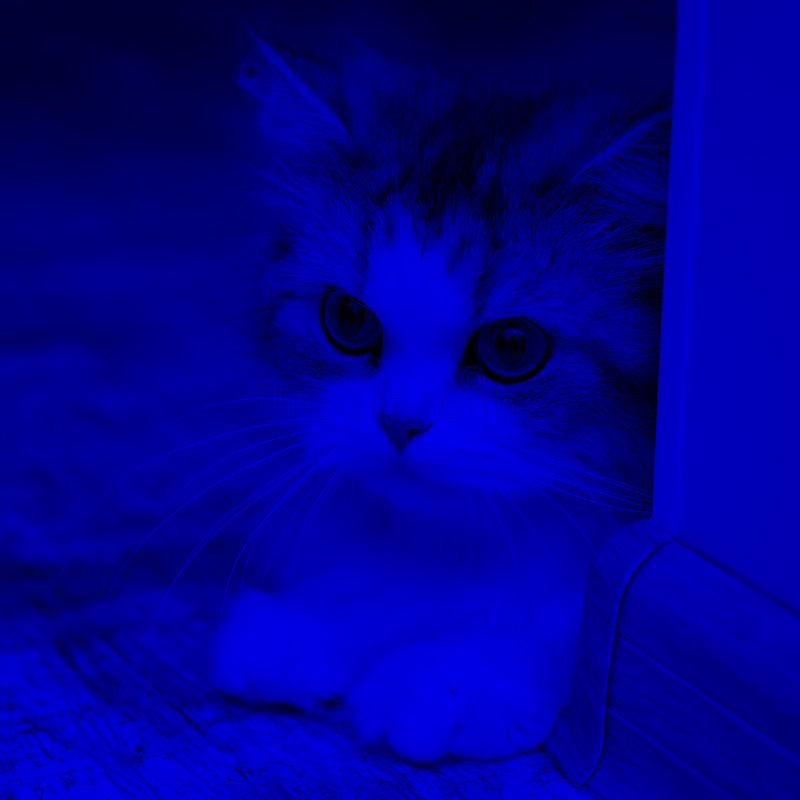
\includegraphics[width=3cm]{data/blue.png}
				};
				\node[] (green) at (-3, 0) {
					
\includegraphics[width=3cm]{data/green.png}
				};
				\node[] (red) at (-3.25, 0.25) {
					
\includegraphics[width=3cm]{data/red.png}
				};

				\draw[<->] ($ (red.north west) - (0.1, 0.1) $) -- ($ (red.south west) - (0.1, -0.1) $) node[midway, above, rotate=90] {\footnotesize{høyde}};
				\draw[<->] ($ (blue.south west) - (-0.1, 0.1) $) -- ($ (blue.south east) - (0.1, 0.1) $) node[midway, below] {\footnotesize{bredde}};
				\draw[<->] ($ (red.north east) + (-0.1, 0.2) $) -- ($ (blue.north east) + (0.2, -0.1) $) node[midway, above, rotate=315] {\footnotesize{kanaler}};
			}
			\visible<4-5>{
				\draw[
					{Stealth[length=5mm]}-{Stealth[length=5mm]},
					double distance=3pt,
					line width=1pt
				] ($ (cat.west) + (-0.4, 0) $) -- ($ (green.east) + (0.65, 0) $);
			}
			\visible<5>{
				\matrix[
					matrix of nodes,
					nodes={
						draw=black,
						fill=white,
						minimum width=0.6cm,
						minimum height=0.6cm,
						anchor=center,
						font=\small\selectfont
					},
					row sep=0cm,
					column sep=0cm
				]  at (-2.75, -0.25) {
					$x_{002}$ \& $x_{012}$ \& $x_{022}$ \& $x_{032}$ \& $x_{042}$ \\
					$x_{102}$ \& $x_{112}$ \& $x_{122}$ \& $x_{132}$ \& $x_{142}$ \\
					$x_{202}$ \& $x_{212}$ \& $x_{222}$ \& $x_{232}$ \& $x_{242}$ \\
					$x_{302}$ \& $x_{312}$ \& $x_{322}$ \& $x_{332}$ \& $x_{342}$ \\
					$x_{402}$ \& $x_{412}$ \& $x_{422}$ \& $x_{432}$ \& $x_{442}$ \\
				};
				\matrix[
					matrix of nodes,
					nodes={
						draw=black,
						fill=white,
						minimum width=0.6cm,
						minimum height=0.6cm,
						anchor=center,
						font=\small\selectfont
					},
					row sep=0cm,
					column sep=0cm
				]  at (-3, 0) {
					$x_{001}$ \& $x_{011}$ \& $x_{021}$ \& $x_{031}$ \& $x_{041}$ \\
					$x_{101}$ \& $x_{111}$ \& $x_{121}$ \& $x_{131}$ \& $x_{141}$ \\
					$x_{201}$ \& $x_{211}$ \& $x_{221}$ \& $x_{231}$ \& $x_{241}$ \\
					$x_{301}$ \& $x_{311}$ \& $x_{321}$ \& $x_{331}$ \& $x_{341}$ \\
					$x_{401}$ \& $x_{411}$ \& $x_{421}$ \& $x_{431}$ \& $x_{441}$ \\
				};
				\matrix[
					matrix of nodes,
					nodes={
						draw=black,
						fill=white,
						minimum width=0.6cm,
						minimum height=0.6cm,
						anchor=center,
						font=\small\selectfont
					},
					row sep=0cm,
					column sep=0cm
				]  at (-3.25, 0.25) {
					$x_{000}$ \& $x_{010}$ \& $x_{020}$ \& $x_{030}$ \& $x_{040}$ \\
					$x_{100}$ \& $x_{110}$ \& $x_{120}$ \& $x_{130}$ \& $x_{140}$ \\
					$x_{200}$ \& $x_{210}$ \& $x_{220}$ \& $x_{230}$ \& $x_{240}$ \\
					$x_{300}$ \& $x_{310}$ \& $x_{320}$ \& $x_{330}$ \& $x_{340}$ \\
					$x_{400}$ \& $x_{410}$ \& $x_{420}$ \& $x_{430}$ \& $x_{440}$ \\
				};
			}
			\visible<6>{
				\node[inner sep=0pt, draw=black] (cat) at (-3.5, 0) {
					
\includegraphics[width=2cm]{data/cat.png}
				};

				\draw[->] (cat) -- (n00);
				\draw[->] (cat) -- (n01);
				\draw[->] (cat) -- (n02);
			}
		\end{tikzpicture}
	\end{frame}

	\begin{frame}{Konvolusjonelle nevrale nettverk: Klassifikasjonsoutput}
		\centering
		\begin{tikzpicture}
			\node[] at (-5.25, -3.5) {};
			\node[] at (5.25, 3.5) {};

			\visible<1-4>{
				\node[inner sep=0pt, draw=black] (cat) at (-3.5, 0) {
					
\includegraphics[width=2cm]{data/cat.png}
				};

				\node[
					circle,
					draw=black,
					fill=green!20,
					minimum size=\nodesize,
					inner sep=0pt
				] (n00) at (-1, 1) {};
				\node[
					circle,
					draw=black,
					fill=green!20,
					minimum size=\nodesize,
					inner sep=0pt
				] (n01) at (-1, 0) {};
				\node[
					circle,
					draw=black,
					fill=green!20,
					minimum size=\nodesize,
					inner sep=0pt
				] (n02) at (-1, -1) {};

				\node[
					circle,
					draw=black,
					fill=green!20,
					minimum size=\nodesize,
					inner sep=0pt
				] (n10) at (1, 1) {};

				\node[
					circle,
					draw=black,
					fill=green!20,
					minimum size=\nodesize,
					inner sep=0pt
				] (n11) at (1, 0) {};
				\node[
					circle,
					draw=black,
					fill=green!20,
					minimum size=\nodesize,
					inner sep=0pt
				] (n12) at (1, -1) {};

				\draw[->] (cat) -- (n00);
				\draw[->] (cat) -- (n01);
				\draw[->] (cat) -- (n02);

				\draw[->] (n00) -- (n10);
				\draw[->] (n00) -- (n11);
				\draw[->] (n00) -- (n12);
				\draw[->] (n01) -- (n10);
				\draw[->] (n01) -- (n11);
				\draw[->] (n01) -- (n12);
				\draw[->] (n02) -- (n10);
				\draw[->] (n02) -- (n11);
				\draw[->] (n02) -- (n12);
			}
			\visible<1>{
				\node[
					circle,
					draw=black,
					fill=green!20,
					minimum size=\nodesize,
					inner sep=0pt,
					text depth=0
				] (y) at (3, 0) {\footnotesize{$y$}};

				\draw[->] (n10) -- (y);
				\draw[->] (n11) -- (y);
				\draw[->] (n12) -- (y);

				\draw[red, very thick] ($ (y.north west) + (-0.2, 0.2) $) -- ($ (y.north east) + (0.2, 0.2) $) -- ($ (y.south east) + (0.2, -0.2) $) -- ($ (y.south west) + (-0.2, -0.2) $) -- cycle;
			}
			\visible<2-3>{
				\node[
					circle,
					draw=black,
					fill=green!20,
					minimum size=\nodesize,
					inner sep=0pt,
					text depth=0
				] (catpred) at (3, 0.5) {\footnotesize{$y_0$}};

				\node[
					circle,
					draw=black,
					fill=green!20,
					minimum size=\nodesize,
					inner sep=0pt,
					text depth=0
				] (dogpred) at (3, -0.5) {\footnotesize{$y_1$}};
			}
			\visible<2-4>{
				\draw[->] (n10) -- (catpred);
				\draw[->] (n11) -- (catpred);
				\draw[->] (n12) -- (catpred);
				\draw[->] (n10) -- (dogpred);
				\draw[->] (n11) -- (dogpred);
				\draw[->] (n12) -- (dogpred);
			}
			\visible<3-4>{
				\node[
					circle,
					draw=black,
					fill=green!20,
					minimum size=\nodesize,
					inner sep=0pt,
					text depth=0,
					label={[text depth=0]right:\small{Cat}}
				] (catpred) at (3, 0.5) {\footnotesize{$y_0$}};

				\node[
					circle,
					draw=black,
					fill=green!20,
					minimum size=\nodesize,
					inner sep=0pt,
					text depth=0,
					label={[text depth=0]right:\small{Dog}}
				] (dogpred) at (3, -0.5) {\footnotesize{$y_1$}};
			}
			\visible<4>{
				\node[font=\Large\selectfont] at (0, -2.5) {
					$\text{kost}=-\sum\limits_i y_i \log(\hat{y}_i)$
				};
			}
		\end{tikzpicture}
	\end{frame}

	\begin{frame}{Konvolusjonelle nevrale nettverk: Arkitektur}
		\centering
		\resizebox{\textwidth}{!}{
			\begin{tikzpicture}
				\node[inner sep=0pt, draw=black] (cat) at (0, 0) {
					
\includegraphics[width=1cm]{data/cat.png}
				};

				\cnnlayer{1.36+0.3}{0}{8}{3}{n1}
				\draw[-stealth] (cat) -- ($ (n1284.south west) - (0.1, 0) $);
				\cnnlayer{2.92+0.3}{0}{6}{3}{n2}
				\draw[-stealth] ($ (n1214.south east) + (0.1, 0) $) -- ($ (n2263.south west) - (0.1, 0) $);
				\cnnlayer{4.43+0.3}{0}{6}{5}{n3}
				\draw[-stealth] ($ (n2213.south east) + (0.1, 0) $) -- ($ (n3363.south west) - (0.2, 0) $);
				\cnnlayer{5.89+0.3}{0}{4}{5}{n4}
				\draw[-stealth] ($ (n3313.south east) + (0.2, 0) $) -- ($ (n4342.south west) - (0.2, 0) $);
				\cnnlayer{7.3+0.3}{0}{4}{7}{n5}
				\draw[-stealth] ($ (n4312.south east) + (0.2, 0) $) -- ($ (n5442.south west) - (0.3, 0) $);
				\cnnlayer{8.66}{0.15}{1}{7}{n6}
				\draw[-stealth] ($ (n5412.south east) + (0.3, 0) $) -- ($ (n6411.south west) - (0, 0) $);

				\node[circle, draw=black, fill=green!20, text depth=0, inner sep=2pt] (y1) at (9.32, 0.275) {\tiny{$y_0$}};
				\node[circle, draw=black, fill=green!20, text depth=0, inner sep=2pt] (y2) at (9.57, 0.025) {\tiny{$y_1$}};

				\foreach \n in {1,...,7}{
					\draw[-stealth] (n6\n11) -- (y1);
					\draw[-stealth] (n6\n11) -- (y2);
				}

				\def\operationfont{\scriptsize}
				\node[text depth=0, font=\operationfont\selectfont, anchor=north] at ($(cat)!0.5!(n1244) + (0, -0.8) $) {Konvolusjon};
				\node[text depth=0, font=\operationfont\selectfont, align=center, anchor=north] at ($(n1244)!0.5!(n2233) + (0, -0.8) $) {Sammenslåing\\(Pooling)};
				\node[text depth=0, font=\operationfont\selectfont, anchor=north] at ($(n2233)!0.5!(n3333) + (0, -0.8) $) {Konvolusjon};
				\node[text depth=0, font=\operationfont\selectfont, align=center, anchor=north] at ($(n3333)!0.5!(n4322) + (0, -0.8) $) {Sammenslåing\\(Pooling)};
				\node[text depth=0, font=\operationfont\selectfont, anchor=north] at ($(n4322)!0.5!(n5422) + (0, -0.8) $) {Konvolusjon};
				\node[text depth=0, font=\operationfont\selectfont, align=center, anchor=north] at ($(n5422)!0.5!(n6411) + (0, -0.8) $) {Sammenslåing\\(Pooling)};
			\end{tikzpicture}
		}
		\vfill
	\end{frame}

	\begin{frame}{Konvolusjonelle nevrale nettverk: Konvolusjon}
		\centering
		\vfill
		\begin{tikzpicture}[
			ampersand replacement=\&
		]
			\matrix[
				every node/.style={
					minimum height=0.6cm,
					minimum width=0.6cm,
					draw=black
				},
				label=\footnotesize{Bilde}
			] (image) at (0, 0) {
				\only<3>{\node[draw=red,fill=white]{};}
				\only<1-2,4->{\node[fill=white]{};} \&
				\only<3-4>{\node[draw=red,fill=black] {};}
				\only<1-2,5->{\node[fill=black] {};} \&
				\only<3-5>{\node[draw=red,fill=black] {};}
				\only<1-2,6->{\node[fill=black] {};} \&
				\only<4-5>{\node[draw=red,fill=black] {};}
				\only<1-3,6->{\node[fill=black] {};} \&
				\only<5>{\node[draw=red,fill=white] {};}
				\only<1-4,6->{\node[fill=white] {};}\\

				\only<3,6>{\node[draw=red,fill=black] {};}
				\only<1-2,4-5,7->{\node[fill=black] {};}  \&
				\only<3-4,6>{\node[draw=red,fill=white] {};}
				\only<1-2,5,7->{\node[fill=white] {};} \&
				\only<3-6>{\node[draw=red,fill=black] {};}
				\only<1-2,7->{\node[fill=black] {};} \&
				\only<4-5>{\node[draw=red,fill=white] {};}
				\only<1-3,6->{\node[fill=white] {};} \&
				\only<5>{\node[draw=red,fill=black] {};}
				\only<1-4,6->{\node[fill=black] {};} \\

				\only<3,6>{\node[draw=red,fill=black] {};}
				\only<1-2,4-5,7->{\node[fill=black] {};} \&
				\only<3-4,6>{\node[draw=red,fill=black] {};}
				\only<1-2,5,7->{\node[fill=black] {};} \&
				\only<3-6>{\node[draw=red,fill=white] {};}
				\only<1-2,7->{\node[fill=white] {};} \&
				\only<4-5>{\node[draw=red,fill=black] {};}
				\only<1-3,6->{\node[fill=black] {};} \&
				\only<5>{\node[draw=red,fill=black] {};}
				\only<1-4,6->{\node[fill=black] {};} \\

				\only<6>{\node[draw=red,fill=black] {};}
				\only<1-5,7->{\node[fill=black] {};} \&
				\only<6>{\node[draw=red,fill=white] {};}
				\only<1-5,7->{\node[fill=white] {};} \&
				\only<6>{\node[draw=red,fill=black] {};}
				\only<1-5,7->{\node[fill=black] {};} \&
				\node[fill=white] {}; \&
				\node[fill=black] {}; \\

				\node[fill=white] {}; \&
				\node[fill=black] {}; \&
				\node[fill=black] {}; \&
				\node[fill=black] {}; \&
				\node[fill=white] {}; \\
			};

			\visible<2->{
				\matrix[
					every node/.style={
						minimum height=0.6cm,
						minimum width=0.6cm,
						draw=black
					},
					label=below:\footnotesize{Mønster 1}] (kernel1) at (-2.25, -3) {
					\only<3-6>{\node[draw=red,fill=white] {};}
					\only<2,7->{\node[fill=white] {};} \&
					\only<3-6>{\node[draw=red,fill=black] {};}
					\only<2,7->{\node[fill=black] {};} \&
					\only<3-6>{\node[draw=red,fill=black] {};}
					\only<2,7->{\node[fill=black] {};} \\

					\only<3-6>{\node[draw=red,fill=black] {};}
					\only<2,7->{\node[fill=black] {};} \&
					\only<3-6>{\node[draw=red,fill=white] {};}
					\only<2,7->{\node[fill=white] {};} \&
					\only<3-6>{\node[draw=red,fill=black] {};}
					\only<2,7->{\node[fill=black] {};} \\

					\only<3-6>{\node[draw=red,fill=black] {};}
					\only<2,7->{\node[fill=black] {};} \&
					\only<3-6>{\node[draw=red,fill=black] {};}
					\only<2,7->{\node[fill=black] {};} \&
					\only<3-6>{\node[draw=red,fill=white] {};}
					\only<2,7->{\node[fill=white] {};} \\
				};
			}
			\visible<3->{
				\matrix[
					nodes in empty cells,
					every node/.style={
						minimum height=0.6cm,
						minimum width=0.6cm
					}
				] (map1) at (5.1, -1.1) {
					\only<3>{\node[draw=red] {3};}
					\only<4->{\node[draw=black] {3};} \&
					\only<4>{\node[draw=red] {0};}
					\only<5->{\node[draw=black] {0};} \&
					\only<5>{\node[draw=red] {1};}
					\only<6->{\node[draw=black] {1};} \\

					\only<6>{\node[draw=red] {0};}
					\only<7->{\node[draw=black] {0};} \&
					\only<7->{\node[draw=black] {3};} \&
					\only<7->{\node[draw=black] {0};} \\

					\only<7->{\node[draw=black] {1};} \&
					\only<7->{\node[draw=black] {0};} \&
					\only<7->{\node[draw=black] {3};} \\
				};
			}
			\visible<8->{
				\matrix[
					every node/.style={
						minimum height=0.6cm,
						minimum width=0.6cm,
						draw=black
					},
					label=below:\footnotesize{Mønster 2}
				] (kernel2) at (0, -3) {
					\node[fill=black] {}; \&
					\node[fill=black] {}; \&
					\node[fill=white] {}; \\

					\node[fill=black] {}; \&
					\node[fill=white] {}; \&
					\node[fill=black] {}; \\

					\node[fill=white] {}; \&
					\node[fill=black] {}; \&
					\node[fill=black] {}; \\
				};

				\matrix[
					every node/.style={
						minimum height=0.6cm,
						minimum width=0.6cm,
						draw=black
					}
				] (map2) at (5.3, -1.3) {
					\node[fill=white] {1}; \&
					\node[fill=white] {0}; \&
					\node[fill=white] {3}; \\

					\node[fill=white] {0}; \&
					\node[fill=white] {3}; \&
					\node[fill=white] {0}; \\

					\node[fill=white] {3}; \&
					\node[fill=white] {0}; \&
					\node[fill=white] {1}; \\
				};
			}
			\visible<9->{
				\matrix[
					every node/.style={
						minimum height=0.6cm,
						minimum width=0.6cm,
						draw=black
					},
					label=below:\footnotesize{Mønster 3}
				] (kernel3) at (2.25, -3) {
					\node[fill=white] {}; \&
					\node[fill=black] {}; \&
					\node[fill=white] {}; \\

					\node[fill=black] {}; \&
					\node[fill=white] {}; \&
					\node[fill=black] {}; \\

					\node[fill=white] {}; \&
					\node[fill=black] {}; \&
					\node[fill=white] {};\\
				};

				\matrix[
					every node/.style={
						minimum height=0.6cm,
						minimum width=0.6cm,
						draw=black
					}
				] (map3) at (5.5, -1.5) {
					\node[fill=white] {3}; \&
					\node[fill=white] {0}; \&
					\node[fill=white] {3}; \\

					\node[fill=white] {0}; \&
					\node[fill=white] {5}; \&
					\node[fill=white] {0}; \\

					\node[fill=white] {3}; \&
					\node[fill=white] {0}; \&
					\node[fill=white] {3}; \\
				};
			}
			\visible<10->{
				\node[anchor=south] at ($ (map1.north) + (0, 0.0) $) {\footnotesize{Feature-kart}};
			}
			\visible<11->{
				\draw[] ($ (kernel1.north west) + (-0.2, 0.2) $) --
						($ (kernel3.north east) + (0.2, 0.2) $) --
						($ (kernel3.south east) + (0.2, -0.5) $) --
						($ (kernel1.south west) + (-0.2, -0.5) $) --
						cycle;
	 			\node[anchor=north] at ($ (kernel2.south) + (0, -0.5) $) {\footnotesize{Vekter/parametre}};
			}
			\visible<12>{
				\matrix[every node/.style={minimum height=0.6cm, minimum width=0.6cm, draw=black}] (map1) at (5.1, -1.1) {
					\node[fill=red!30] {};  \& \node[fill=white] {}; \& \node[fill=red!10] {};\\
					\node[fill=white] {};  \& \node[fill=red!30] {}; \& \node[fill=white] {};\\
					\node[fill=red!10] {};  \& \node[fill=white] {}; \& \node[fill=red!30] {};\\
				};

				\matrix[every node/.style={minimum height=0.6cm, minimum width=0.6cm, draw=black}] (map2) at (5.3, -1.3) {
					\node[fill=green!10] {};  \& \node[fill=white] {}; \& \node[fill=green!30] {};\\
					\node[fill=white] {};  \& \node[fill=green!30] {}; \& \node[fill=white] {};\\
					\node[fill=green!30] {};  \& \node[fill=white] {}; \& \node[fill=green!10] {};\\
				};

				\matrix[every node/.style={minimum height=0.6cm, minimum width=0.6cm, draw=black}] (map3) at (5.5, -1.5) {
					\node[fill=blue!30] {};  \& \node[fill=white] {}; \& \node[fill=blue!30] {};\\
					\node[fill=white] {};  \& \node[fill=blue!50] {}; \& \node[fill=white] {};\\
					\node[fill=blue!30] {};  \& \node[fill=white] {}; \& \node[fill=blue!30] {};\\
				};
			}
		\end{tikzpicture}
	\end{frame}

	\begin{frame}{Konvolusjonelle nevrale nettverk: Pooling}
		\centering
		\vfill
		\begin{tikzpicture}[
			ampersand replacement=\&
		]
			\node[] at (-2, 0) {};
			\node[] at (4.2, 0) {};

			\matrix[
				every node/.style={
					minimum height=0.8cm,
					minimum width=0.8cm,
					draw=black
				},
				label=\footnotesize{Feature-kart}
			] (image) at (0, 0) {
				\only<2>{\node[draw=red] {0};}
				\only<1,3->{\node[] {0};} \&
				\only<2>{\node[draw=red] {1};}
				\only<1,3->{\node[] {1};} \&
				\only<3>{\node[draw=red] {2};}
				\only<1-2,4->{\node[] {2};} \&
				\only<3>{\node[draw=red] {3};}
				\only<1-2,4->{\node[] {3};} \\

				\only<2>{\node[draw=red] {4};}
				\only<1,3->{\node[] {4};} \&
				\only<2>{\node[draw=red] {5};}
				\only<1,3->{\node[] {5};} \&
				\only<3>{\node[draw=red] {6};}
				\only<1-2,4->{\node[] {6};} \&
				\only<3>{\node[draw=red] {7};}
				\only<1-2,4->{\node[] {7};} \\

				\only<4>{\node[draw=red] {8};}
				\only<1-3,5->{\node[] {8};} \&
				\only<4>{\node[draw=red] {9};}
				\only<1-3,5->{\node[] {9};} \&
				\only<5>{\node[draw=red] {10};}
				\only<1-4,6->{\node[] {10};} \&
				\only<5>{\node[draw=red] {11};}
				\only<1-4,6->{\node[] {1};} \\

				\only<4>{\node[draw=red] {12};}
				\only<1-3,5->{\node[] {12};} \&
				\only<4>{\node[draw=red] {13};}
				\only<1-3,5->{\node[] {13};} \&
				\only<5>{\node[draw=red] {14};}
				\only<1-4,6->{\node[] {14};} \&
				\only<5>{\node[draw=red] {15};}
				\only<1-4,6->{\node[] {15};} \\
			};

			\matrix[
				every node/.style={
					minimum height=0.8cm,
					minimum width=0.8cm
				}
			] (map) at ($ (image) + (3, 0) $) {
				\only<2>{\node[draw=red] {5};}
				\only<3->{\node[draw=black] {5};}\&
				\only<3>{\node[draw=red] {7};}
				\only<4->{\node[draw=black] {7};} \\

				\only<4>{\node[draw=red] {13};}
				\only<5->{\node[draw=black] {13};} \&
				\only<5>{\node[draw=red] {15};}
				\only<6->{\node[draw=black] {15};} \\
			};
		\end{tikzpicture}
		\vfill
	\end{frame}

	\begin{frame}{Konvolusjonelle nevrale nettverk: Arkitektur}
		\centering
		\resizebox{\textwidth}{!}{
			\begin{tikzpicture}
				\only<1-2>{
					\node[inner sep=0pt, draw=black] (cat) at (0, 0) {
						
\includegraphics[width=1cm]{data/cat.png}
					};

					\cnnlayer{1.36+0.3}{0}{8}{3}{n1}
					\draw[-stealth] (cat) -- ($ (n1284.south west) - (0.1, 0) $);
					\cnnlayer{2.92+0.3}{0}{6}{3}{n2}
					\draw[-stealth] ($ (n1214.south east) + (0.1, 0) $) -- ($ (n2263.south west) - (0.1, 0) $);
					\cnnlayer{4.43+0.3}{0}{6}{5}{n3}
					\draw[-stealth] ($ (n2213.south east) + (0.1, 0) $) -- ($ (n3363.south west) - (0.2, 0) $);
					\cnnlayer{5.89+0.3}{0}{4}{5}{n4}
					\draw[-stealth] ($ (n3313.south east) + (0.2, 0) $) -- ($ (n4342.south west) - (0.2, 0) $);
					\cnnlayer{7.3+0.3}{0}{4}{7}{n5}
					\draw[-stealth] ($ (n4312.south east) + (0.2, 0) $) -- ($ (n5442.south west) - (0.3, 0) $);
					\cnnlayer{8.66}{0.15}{1}{7}{n6}
					\draw[-stealth] ($ (n5412.south east) + (0.3, 0) $) -- ($ (n6411.south west) - (0, 0) $);

					\node[circle, draw=black, fill=green!20, text depth=0, inner sep=2pt] (y1) at (9.32, 0.275) {\tiny{$y_0$}};
					\node[circle, draw=black, fill=green!20, text depth=0, inner sep=2pt] (y2) at (9.57, 0.025) {\tiny{$y_1$}};

					\only<1>{
						\foreach \n in {1,...,7}{
							\draw[-stealth] (n6\n11) -- (y1);
							\draw[-stealth] (n6\n11) -- (y2);
						}
					}
					\only<2>{
						\foreach \n in {1,...,7}{
							\draw[red, -stealth] (n6\n11) -- (y1);
							\draw[red, -stealth] (n6\n11) -- (y2);
						}
					}

					\def\operationfont{\scriptsize}
					\node[text depth=0, font=\operationfont\selectfont, anchor=north] at ($(cat)!0.5!(n1244) + (0, -0.8) $) {Konvolusjon};
					\node[text depth=0, font=\operationfont\selectfont, align=center, anchor=north] at ($(n1244)!0.5!(n2233) + (0, -0.8) $) {Sammenslåing\\(Pooling)};
					\node[text depth=0, font=\operationfont\selectfont, anchor=north] at ($(n2233)!0.5!(n3333) + (0, -0.8) $) {Konvolusjon};
					\node[text depth=0, font=\operationfont\selectfont, align=center, anchor=north] at ($(n3333)!0.5!(n4322) + (0, -0.8) $) {Sammenslåing\\(Pooling)};
					\node[text depth=0, font=\operationfont\selectfont, anchor=north] at ($(n4322)!0.5!(n5422) + (0, -0.8) $) {Konvolusjon};
					\node[text depth=0, font=\operationfont\selectfont, align=center, anchor=north] at ($(n5422)!0.5!(n6411) + (0, -0.8) $) {Sammenslåing\\(Pooling)};


					\node[text depth=0] at ($(cat)!0.5!(n1244) + (0, -3) $) {
						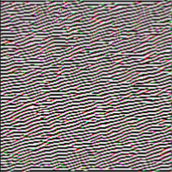
\includegraphics[height=2cm, width=2cm]{data/first.png}
					};

					\node[text depth=0] at ($(n2233)!0.5!(n3333) + (0, -3) $) {
						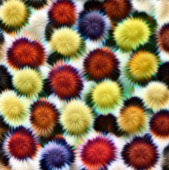
\includegraphics[height=2cm, width=2cm]{data/third.png}
					};

					\node[text depth=0] at ($(n4322)!0.5!(n5422) + (0, -3) $) {
						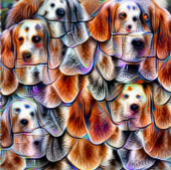
\includegraphics[height=2cm, width=2cm]{data/fifth.png}
					};
				}
				\visible<3>{
					\node[inner sep=0pt, draw=black] at (4.6, -1) {
						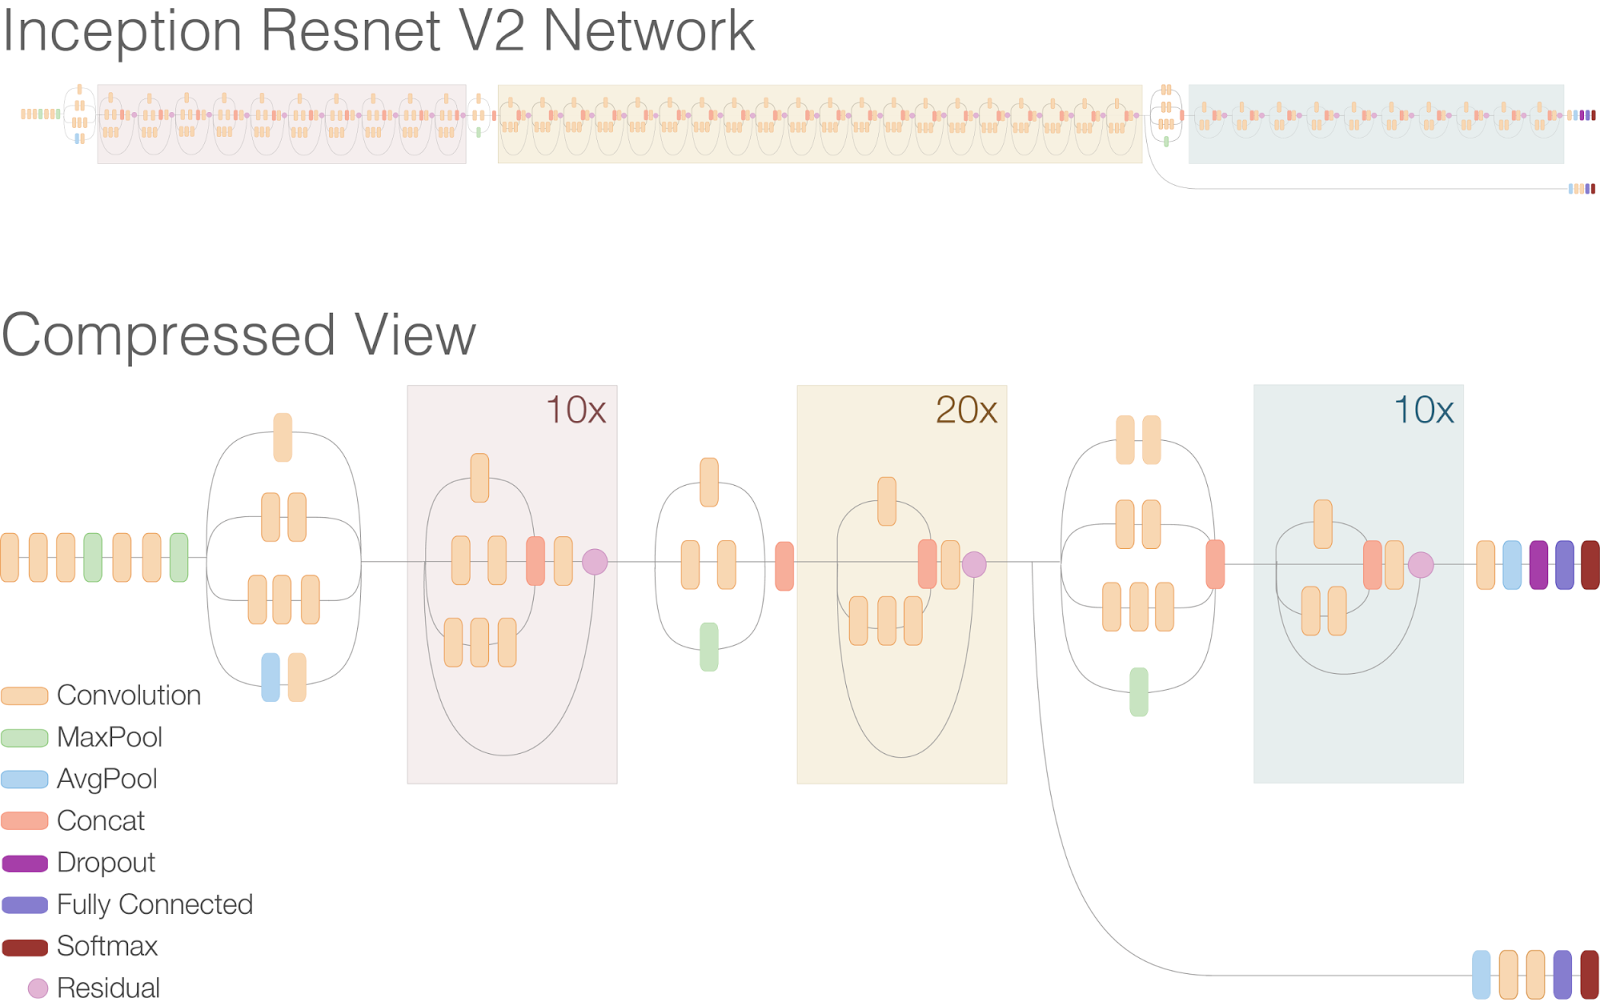
\includegraphics[width=8cm]{data/inception.png}
					};
				}
				\only<4>{
					\node[text width=10cm, align=left] at (4.6, -1) {
						\textbf{Hvordan fungerer et konvolusjonelt nevralt nettverk (for klassifikasjon)?}\\
						\begin{itemize}
							\item Bilder representeres ved 3-dimensjonale arrayer i en datamaskin, som kan mates direkte som input til nettverket
							\item For å oppnå klassifikasjon gir vi nettverket flere output-nevroner, en for hver klasse vi er interessert i, også tolker vi outputen slik at nevronet med høyest verdi sammensvarer med den predikerte klassifikatoren
							\item Inne i nettverket utføres alternerende konvolusjoner og pooling som i praksis lar oss gjenkjenne større og mer abstrakte mønstre jo dypere i modellen vi kommer
							\item Til slutt kobles mønstrene opp mot klassene ved et "vanlig" nevralt nett (alle-til-alle koblinger)
							\item Parametrene som trenes ligger i konvolusjonene og sier hvilke mønstre som må læres, og i det siste laget
						\end{itemize}
					};
				}
			\end{tikzpicture}
		}
	\end{frame}

	\section{Praktiske tips}

	\begin{frame}{Praktiske tips: Transfer learning}
		\centering
		\resizebox{\textwidth}{!}{
			\begin{tikzpicture}
				\only<1-4>{
					\node[inner sep=0pt, draw=black] (cat) at (0, 0) {
						
\includegraphics[width=1cm]{data/cat.png}
					};

					\cnnlayer{1.36+0.3}{0}{8}{3}{n1}
					\draw[-stealth] (cat) -- ($ (n1284.south west) - (0.1, 0) $);
					\cnnlayer{2.92+0.3}{0}{6}{3}{n2}
					\draw[-stealth] ($ (n1214.south east) + (0.1, 0) $) -- ($ (n2263.south west) - (0.1, 0) $);
					\cnnlayer{4.43+0.3}{0}{6}{5}{n3}
					\draw[-stealth] ($ (n2213.south east) + (0.1, 0) $) -- ($ (n3363.south west) - (0.2, 0) $);
					\cnnlayer{5.89+0.3}{0}{4}{5}{n4}
					\draw[-stealth] ($ (n3313.south east) + (0.2, 0) $) -- ($ (n4342.south west) - (0.2, 0) $);
					\cnnlayer{7.3+0.3}{0}{4}{7}{n5}
					\draw[-stealth] ($ (n4312.south east) + (0.2, 0) $) -- ($ (n5442.south west) - (0.3, 0) $);
					\cnnlayer{8.66}{0.15}{1}{7}{n6}
					\draw[-stealth] ($ (n5412.south east) + (0.3, 0) $) -- ($ (n6411.south west) - (0, 0) $);

					\visible<1>{
						\node[circle, draw=black, fill=green!20, text depth=0, inner sep=2pt, label={[text depth=0pt]right:\tiny{Cat}}] (y1) at (9.32, 0.275) {\tiny{$y_0$}};
						\node[circle, draw=black, fill=green!20, text depth=0, inner sep=2pt, label={[text depth=0pt]right:\tiny{Dog}}] (y2) at (9.57, 0.025) {\tiny{$y_1$}};

						\foreach \n in {1,...,7}{
							\draw[-stealth] (n6\n11) -- (y1);
							\draw[-stealth] (n6\n11) -- (y2);
						}
					}

					\visible<3-4>{
						\node[circle, draw=black, fill=green!20, text depth=0, inner sep=2pt, label={[text depth=0pt]right:\tiny{Prestekrage}}] (y1) at (9.195, 0.4) {\tiny{$y_0$}};
						\node[circle, draw=black, fill=green!20, text depth=0, inner sep=2pt, label={[text depth=0pt]right:\tiny{Hestehov}}] (y2) at (9.445, 0.15) {\tiny{$y_1$}};
						\node[circle, draw=black, fill=green!20, text depth=0, inner sep=2pt, label={[text depth=0pt]right:\tiny{Rose}}] (y3) at (9.695, -0.1) {\tiny{$y_1$}};
					}
					\visible<3>{
						\foreach \n in {1,...,7}{
							\draw[-stealth] (n6\n11) -- (y1);
							\draw[-stealth] (n6\n11) -- (y2);
							\draw[-stealth] (n6\n11) -- (y3);
						}
					}
					\visible<4>{
						\foreach \n in {1,...,7}{
							\draw[red,-stealth] (n6\n11) -- (y1);
							\draw[red,-stealth] (n6\n11) -- (y2);
							\draw[red,-stealth] (n6\n11) -- (y3);
						}
					}

					\node[text depth=0] at ($(cat)!0.5!(n1244) + (0, -3) $) {
						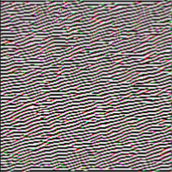
\includegraphics[height=2cm, width=2cm]{data/first.png}
					};

					\node[text depth=0] at ($(n2233)!0.5!(n3333) + (0, -3) $) {
						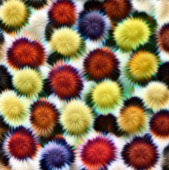
\includegraphics[height=2cm, width=2cm]{data/third.png}
					};

					\node[text depth=0] at ($(n4322)!0.5!(n5422) + (0, -3) $) {
						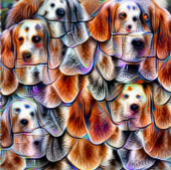
\includegraphics[height=2cm, width=2cm]{data/fifth.png}
					};
				}
				\only<5>{
					\node[text width=10cm, align=left] at (4.6, -1) {
						\textbf{Hva er transfer learning?}\\
						\begin{itemize}
							\item En teknikk for å utnytte at det er overlapp mellom visuelle problemer, og at et nettverk som har blitt trent til å løse èn oppgave antageligvis har lært noe som er nyttig også for en annen
							\item I praksis: Vi beholder de første lagene av en ferdigtrent modell (som gjenkjenner generiske visuelle mønstre, kanter, farger, geometri etc) og trener nye lag på toppen av disse
						\end{itemize}
					};
				}
			\end{tikzpicture}
		}
	\end{frame}

	\newcommand{\overfittingplot}[1]{
		\begin{tikzpicture}
			\begin{axis}[
				xlabel=$m^2$,
				ylabel=NOK,
				ytick={4000000, 5000000, 6000000, 7000000, 8000000},
				yticklabels={4M, 5M, 6M, 7M, 8M},
				scaled y ticks=false,
				xtick pos=bottom,
				ytick pos=left,
				xmin=30,
				xmax=90,,
				ymin=3500000,
				ymax=8800000
			]
				\ifnum#1<4
					\addplot[
						only marks,
						mark size=3pt,
						mark options={draw=black, fill=cyan}
					] coordinates {
						(72, 5127379)
						(50, 4552170)
						(45, 4486654)
						(62, 5709276)
						(53, 4634912)
						(81, 8388570)
						(44, 4828170)
						(78, 7557770)
						(37, 4016520)
						(73, 6572351)
					};

					\ifnum#1>0
						\addplot[smooth] coordinates {
							(36, 3000000)
							(37, 4016520)
							(40, 10000000)
							(44, 4828170)
							(45, 4486654)
							(47, 3900000)
							(50, 4552170)
							(51, 4800000)
							(53, 4634912)
							(57, 4300000)
							(62, 5709276)
							(64, 5500000)
							(71, 2000000)
							(72, 5127379)
							(73, 6572351)
							(78, 7557770)
							(81, 8388570)
							(83, 10000000)
						};
					\fi

					\ifnum#1=2
						\addplot[
							only marks,
							mark size=3pt,
							mark options={draw=black, fill=red}
						] coordinates {
							(40, 4400000)
							(59, 5500000)
							(69, 5900000)
							(85, 7000000)
							(88, 7400000)
						};
					\fi

					\ifnum#1=3
						\addplot[model3, thick] coordinates {
							(0, 706495)
							(100, 8909658)
						};
					\fi
				\fi

				\ifnum#1=4
					\addplot[
						only marks,
						mark size=3pt,
						mark options={draw=black, fill=cyan}
					] table [x=X, y=y, col sep=comma] {data/data.csv};
				\fi

			\end{axis}
		\end{tikzpicture}
	}

	\newsavebox{\overfittingdata}
	\sbox{\overfittingdata}{\overfittingplot{0}}
	\newsavebox{\overfittingtrace}
	\sbox{\overfittingtrace}{\overfittingplot{1}}
	\newsavebox{\overfittingtest}
	\sbox{\overfittingtest}{\overfittingplot{2}}
	\newsavebox{\overfittingregularized}
	\sbox{\overfittingregularized}{\overfittingplot{3}}
	\newsavebox{\overfittingmore}
	\sbox{\overfittingmore}{\overfittingplot{4}}

	\newsavebox{\traintest}
	\sbox{\traintest}{
		\begin{tikzpicture}
			\begin{axis}[
				xmin=0,
				xmax=99,
				ymin=0,
				ymax=100,
				ticks=none,
				xlabel=Tid,
				ylabel=Kost,
				legend cell align={left},
			]
				\addplot[cyan, thick] table[x=epoch, y=train, col sep=comma] {data/losses.csv};
				\addplot[red, thick] table[x=epoch, y=val, col sep=comma] {data/losses.csv};
				\addlegendentry{Treningsdata}
				\addlegendentry{Valideringsdata}
			\end{axis}
		\end{tikzpicture}
	}

	\begin{frame}{Praktiske tips: Overtilpasning}
		\centering
		\begin{tikzpicture}
			\visible<1>{
				\node[] at (0, 0) {
					\usebox{\overfittingdata}
				};
			}
			\visible<2>{
				\node[] at (0, 0) {
					\usebox{\overfittingtrace}
				};
			}
			\visible<3>{
				\node[] at (0, 0) {
					\usebox{\overfittingtest}
				};
			}
			\visible<4>{
				\node[] at (0, 0) {
					\usebox{\traintest}
				};
			}
			\visible<5>{
				\node[] at (0, 0) {
					\usebox{\overfittingmore}
				};
			}
			\visible<6>{
				\node[] at (0, 0) {
					\usebox{\overfittingregularized}
				};
			}
			\visible<7>{
				\node[
					circle,
					draw=black,
					fill=green!20,
					minimum size=\nodesize,
					inner sep=0pt,
					text depth=0
				] (x0) at (-3, 0.5) {\footnotesize{$x_0$}};
				\node[
					circle,
					draw=black,
					fill=green!20,
					minimum size=\nodesize,
					inner sep=0pt,
					text depth=0
				] (x1) at (-3, -0.5) {\footnotesize{$x_1$}};

				\node[
					circle,
					draw=black,
					fill=green!20,
					minimum size=\nodesize,
					inner sep=0pt
				] (n00) at (-1, 1) {};
				\node[
					circle,
					draw=black,
					fill=green!20,
					minimum size=\nodesize,
					inner sep=0pt
				] (n01) at (-1, 0) {};
				\node[
					circle,
					draw=black,
					fill=gray,
					minimum size=\nodesize,
					inner sep=0pt
				] (n02) at (-1, -1) {};

				\node[
					circle,
					draw=black,
					fill=gray,
					minimum size=\nodesize,
					inner sep=0pt
				] (n10) at (1, 1) {};

				\node[
					circle,
					draw=black,
					fill=green!20,
					minimum size=\nodesize,
					inner sep=0pt
				] (n11) at (1, 0) {};
				\node[
					circle,
					draw=black,
					fill=gray,
					minimum size=\nodesize,
					inner sep=0pt
				] (n12) at (1, -1) {};

				\node[
					circle,
					draw=black,
					fill=green!20,
					minimum size=\nodesize,
					inner sep=0pt,
					text depth=0
				] (y) at (3, 0) {\footnotesize{$y$}};

				\draw[->] (x0) -- (n00);
				\draw[->] (x0) -- (n01);
				\draw[->] (x0) -- (n02);
				\draw[->] (x1) -- (n00);
				\draw[->] (x1) -- (n01);
				\draw[->] (x1) -- (n02);

				\draw[->] (n00) -- (n10);
				\draw[->] (n00) -- (n11);
				\draw[->] (n00) -- (n12);
				\draw[->] (n01) -- (n10);
				\draw[->] (n01) -- (n11);
				\draw[->] (n01) -- (n12);
				\draw[->] (n02) -- (n10);
				\draw[->] (n02) -- (n11);
				\draw[->] (n02) -- (n12);

				\draw[->] (n10) -- (y);
				\draw[->] (n11) -- (y);
				\draw[->] (n12) -- (y);
			}
			\visible<8-10>{
				\node[inner sep=0pt, draw=black] (orig) at (-3, 0) {
					
\includegraphics[width=3cm]{data/cat.png}
				};
			}
			\visible<9>{
				\node[inner sep=0pt, draw=black] (rotate) at (3, 2.5) {
					\rotatebox[origin=c]{90}{
\includegraphics[width=2cm]{data/cat.png}}
				};
				\node[inner sep=0pt, draw=black] (flip) at (3, 0) {
					\scalebox{-1}[1]{
\includegraphics[width=2cm]{data/cat.png}}
				};
				\node[inner sep=0pt, draw=black] (zoom) at (3, -2.5) {
					
\includegraphics[
						width=2cm,
						trim={2cm 2cm 2cm 2cm},
						clip
					]{data/cat.png}
				};

				\draw[-stealth, line width=5, blue!50] (orig) -- (rotate);
				\draw[-stealth, line width=5, blue!50] (orig) -- (flip);
				\draw[-stealth, line width=5, blue!50] (orig) -- (zoom);
			}
			\visible<10>{
				\node[inner sep=0pt, draw=black] (zoom) at (3, 0) {
					
\includegraphics[
						width=3cm,
						trim={4.5cm 0.5cm 0.5cm 4.5cm},
						clip
					]{data/cat.png}
				};

				\draw[-stealth, line width=5, red!50] (orig) -- (zoom);
			}
			\only<11>{
				\node[text width=10cm, align=left] at (0, 0) {
					\textbf{Hva er overtilpasning, og hvordan unngår vi det?}\\
					\begin{itemize}
						\item Modellen har lært å gjenkjenne mønstre i treningsdataen som \textbf{ikke holder} i det generelle tilfellet (e.g. i ny data)
						\item Vi unngår det ved: Store datamengder, strikt testing (\textbf{!!!}), regularisering, augmentering, \ldots
					\end{itemize}
				};
			}
		\end{tikzpicture}
	\end{frame}
\end{document}
